\documentclass[a4paper]{article}
\usepackage[T1]{fontenc}			% \chapter package
\usepackage[english]{babel}
\usepackage[english]{isodate}  		% date format
\usepackage{graphicx}				% manage images
\usepackage{amsfonts}
\usepackage{booktabs}				% high quality tables
\usepackage{amsmath}				% math package
\usepackage{amssymb}				% another math package (e.g. \nexists)
\usepackage{bm}                     % bold math symbols
\usepackage{mathtools}				% emphasize equations
\usepackage{stmaryrd} 				% '\llbracket' and '\rrbracket'
\usepackage{amsthm}					% better theorems
\usepackage{enumitem}				% manage list
\usepackage{pifont}					% nice itemize
\usepackage{cancel}					% cancel math equations
\usepackage{caption}				% custom caption
\usepackage[]{mdframed}				% box text
\usepackage{multirow}				% more lines in a table
\usepackage{textcomp, gensymb}		% degree symbol
\usepackage[x11names]{xcolor}		% RGB color
\usepackage{tcolorbox}				% colorful box
\usepackage{multicol}				% more rows in a table (used for the lists)
\usepackage{listings}
\usepackage{url}
\usepackage{qrcode}
\usepackage{fontawesome5}
\usepackage{ragged2e}
\usepackage{cite}                   % references
\usepackage{imakeidx}               % index
\makeindex[program=makeindex, columns=2,
           title=Index, 
           intoc,
           options={-s index-style.ist}]


\definecolor{codegreen}{rgb}{0,0.6,0}
\definecolor{codegray}{rgb}{0.5,0.5,0.5}
\definecolor{codepurple}{rgb}{0.58,0,0.82}
\definecolor{backcolour}{rgb}{0.95,0.95,0.92}
\lstdefinestyle{mystyle}{
    backgroundcolor=\color{backcolour},   
    commentstyle=\color{codegreen},
    keywordstyle=\color{magenta},
    numberstyle=\tiny\color{codegray},
    stringstyle=\color{codepurple},
    basicstyle=\ttfamily\footnotesize,
    breakatwhitespace=false,         
    breaklines=true,                 
    captionpos=b,                    
    keepspaces=true,                 
    numbers=left,                    
    numbersep=5pt,                  
    showspaces=false,                
    showstringspaces=false,
    showtabs=false,                  
    tabsize=2
}
\lstset{style=mystyle}


% draw a frame around given text
\newcommand{\framedtext}[1]{%
	\par%
	\noindent\fbox{%
		\parbox{\dimexpr\linewidth-2\fboxsep-2\fboxrule}{#1}%
	}%
}


% table of content links
\usepackage{xcolor}
\usepackage[linkcolor=black, citecolor=blue, urlcolor=cyan]{hyperref} % hypertexnames=false
\hypersetup{
	colorlinks=true
}


\newtheorem{theorem}{\textcolor{Red3}{\underline{Theorem}}}
\renewcommand{\qedsymbol}{QED}
\newcommand{\dquotes}[1]{``#1''}
\newcommand{\longline}{\noindent\rule{\textwidth}{0.4pt}}
\newcommand{\circledtext}[1]{\raisebox{.5pt}{\textcircled{\raisebox{-.9pt}{#1}}}}
\newcommand{\definition}[1]{\textcolor{Red3}{\textbf{#1}}\index{#1}}
\newcommand{\example}[1]{\textcolor{Green4}{\textbf{#1}}}
\newcommand{\highspace}{\vspace{1.2em}\noindent}


\begin{document}
    \newcounter{definition}[section]
    \newcounter{example}[section]
    
    \newtcolorbox[use counter = definition]{definitionbox}{%
        colback=red!5!white,
        colframe=red!75!black,
        fonttitle=\bfseries,
        title=Definition \thetcbcounter %
    }
    
    \newtcolorbox[use counter = example]{examplebox}{%
        colback=Green4!5!white,
        colframe=Green4!75!black,
        fonttitle=\bfseries,
        title=Example \thetcbcounter %
    }

    \author{260236}
	\title{Software Engineering for HPC - Notes}
	\date{\printdayoff\today}
	\maketitle

	\newpage

    \section*{Preface}

    Every theory section in these notes has been taken from two sources:
    \begin{itemize}
        \item None
    \end{itemize}
    About:
    \begin{itemize}
        \item[\faIcon{github}] \href{https://github.com/AndreVale69/HPC-E-PoliMI-university-notes}{GitHub repository}
    \end{itemize}
    
    \newpage
	
	\tableofcontents

    \newpage

    \section{Introduction}

    \subsection{The importance of software engineering}

    Software engineering is so important because it is everywhere. Our society is now totally dependent on software-intensive systems. Think about it. The society could not function without software, for example:
    \begin{itemize}
        \item Transportation systems;
        \item Energy systems;
        \item Manufacturing systems.
    \end{itemize}
    For these reasons, \textbf{software failures cannot be tolerated}.

    \highspace
    In the following list, we can see some famous software issues:
    \begin{itemize}
        \item \example{911 Outage on April 2014}. On 10th April 2014, Washington State had no 911 service for six hours. A software issue causes this event. The software dispatching the calls had a counter used to assign a unique identifier to each call. The counter went over the threshold defined by developers. All calls from that moment on were rejected.
        
        More info is \href{https://www.theatlantic.com/technology/archive/2017/09/saving-the-world-from-code/540393/}{here}.

        \item \example{Ariane 5, 1996}. On 4th June 1996, forty seconds after take off, Ariane 5 broke up and exploded. The total cost for developing the launcher has been 8000 million dollars. The launcher contained a cluster of satellites for 500 million dollars. Again, the explosion was caused by software failure. 
        
        More info is here: \href{http://sunnyday.mit.edu/accidents/Ariane5accidentreport.html}{accident tech report} and \href{https://www.youtube.com/watch?v=PK_yguLapgA}{video}.
    \end{itemize}

    \newpage

    \subsection{Software engineering: definition}

    There are some fields of computer science dealing with software systems:
    \begin{itemize}
        \item Large and complex;
        \item Built by teams;
        \item It exists in many versions;
        \item Last many years;
        \item Undergo changes.
    \end{itemize}
    In each field, a software engineer needs to have some skills. In contrast to a \emph{programmer} that has the following abilities:
    \begin{itemize}
        \item They develop a complete program;
        \item They work on known specifications;
        \item They work individually.
    \end{itemize}
    A \textbf{software engineer} has the following \textbf{skills}:
    \begin{itemize}
        \item \textbf{Identifies} \emph{requirements} and develops \emph{specifications};
        \item \textbf{Designs} a component to be combined with other components, developed, maintained, and used by others; component can become part of several systems;
        \item \textbf{Works in a team}.
    \end{itemize}
    We can \underline{summarize} the skills of a software engineer as follows:
    \begin{itemize}
        \item Technical
        \item Project management
        \item Cognitive
        \item Enterprise organization
        \item Interaction with different cultures
        \item Domain knowledge
    \end{itemize}
    The \textbf{main goal} of a software engineer is to \textbf{develop software products}. Not only is the product significant, but the \textbf{process is also fundamental}. The quality of the process affects the quality of the product.

    \newpage

    \subsection{The software product and the process}

    The product developed by a software engineer differs from traditional product types. It isn't easy to describe and evaluate because it is intangible. Some \textbf{aspects affecting the product quality}:
    \begin{itemize}
        \item \textbf{Development technology};
        \item \textbf{Process quality};
        \item \textbf{People quality};
        \item \textbf{Cost, time and schedule}.
    \end{itemize}

    \longline

    \subsubsection{ISO/IEC 25010}

    An \href{https://en.wikipedia.org/wiki/International_Organization_for_Standardization}{ISO} (International Organization for Standardization) called \textbf{ISO/IEC 25010} comprises the \textbf{nine quality characteristics}:
    \begin{figure}[!htp]
        \centering
        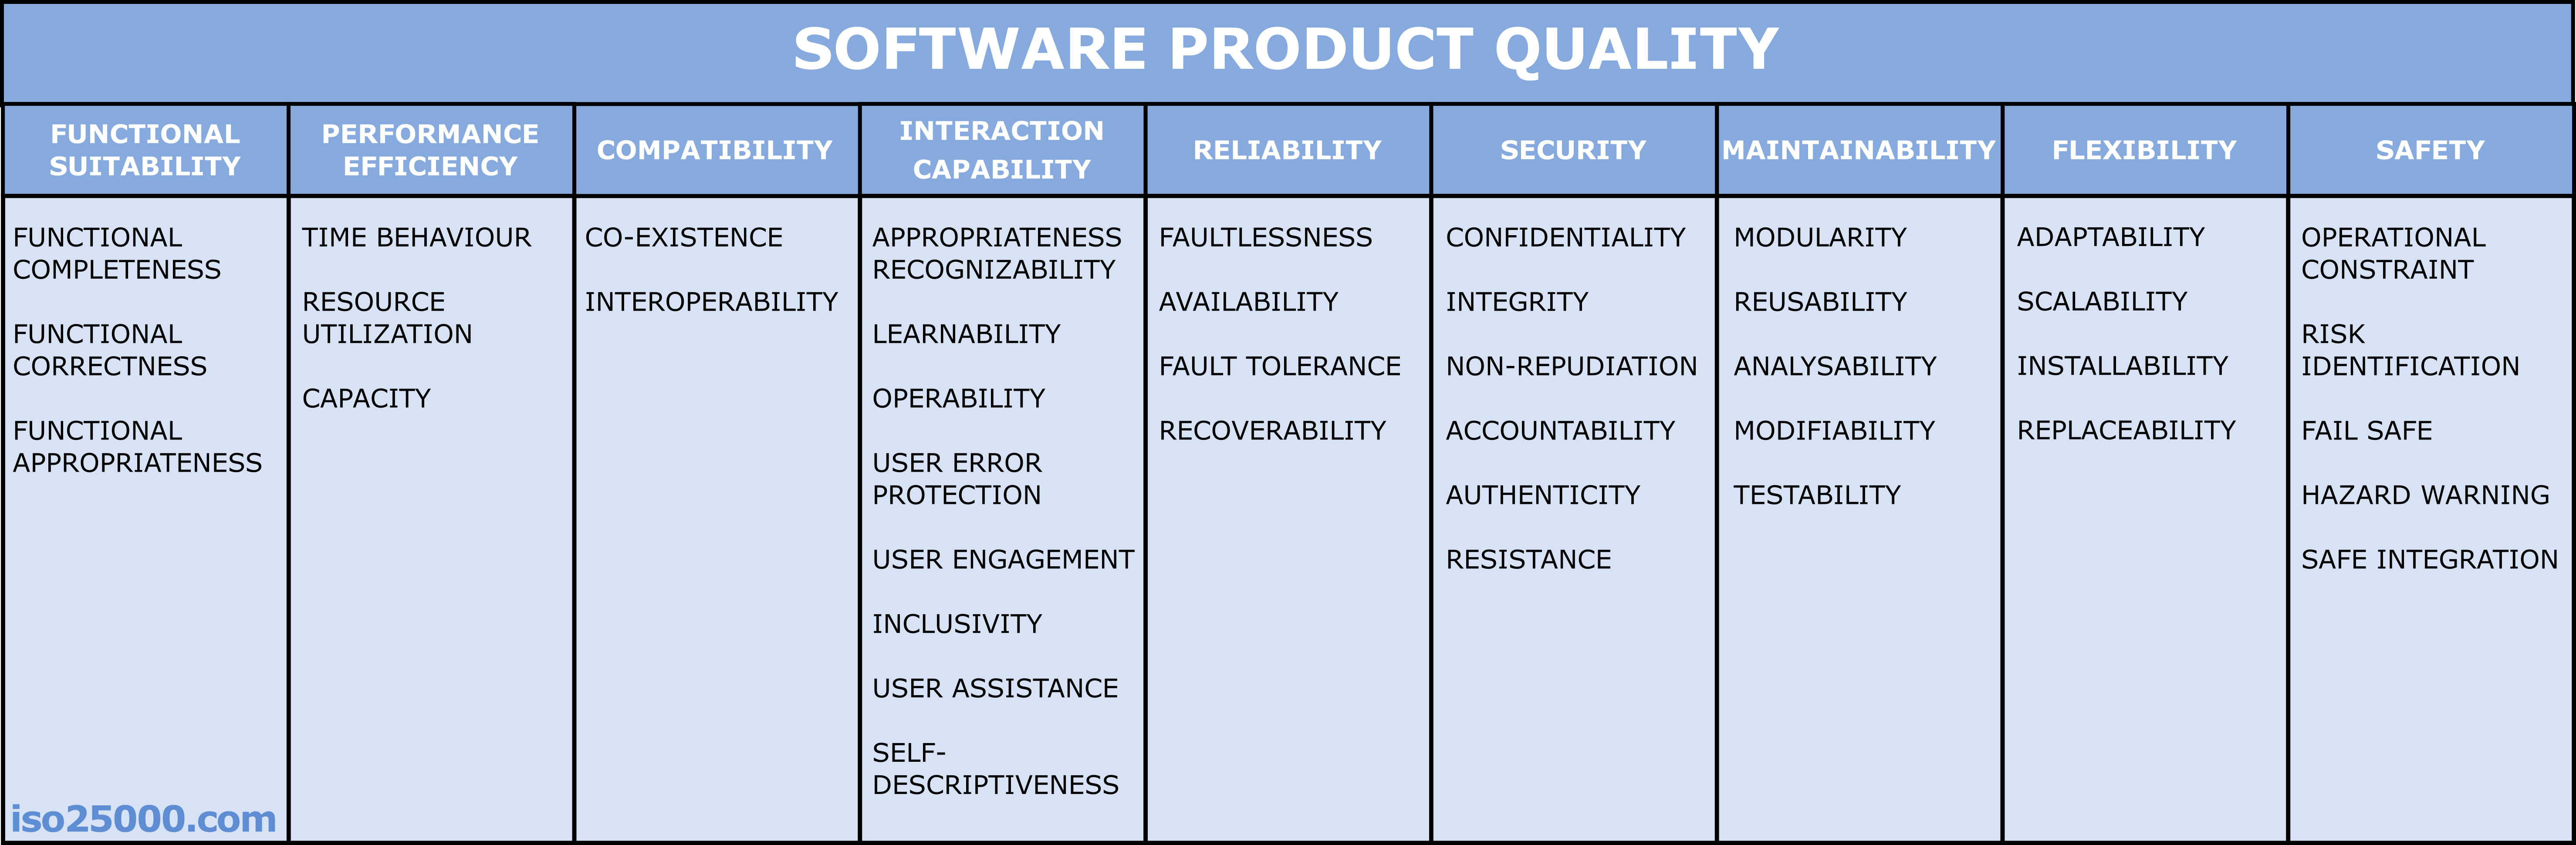
\includegraphics[width=\textwidth]{img/iso_25010_en.png}
        \caption{\href{https://iso25000.com/index.php/en/iso-25000-standards/iso-25010}{ISO/IEC 25010}}
    \end{figure}

    \longline

    \subsubsection{Productivity}

    A process quality to consider is \textbf{productivity} (the \textbf{process of producing a product}). The definition can be: \dquotes{ability to produce a good amount of product}. To \textbf{measure it}, we can use \textbf{delivered items by unit of effort}, where:
    \begin{itemize}
        \item \textbf{Delivered items}: lines of code (and variations) function points;
        \item \textbf{Unit of effort}: person month (note: persons and months cannot be interchanged).
    \end{itemize}

    \newpage

    \subsubsection{Timeliness}

    Another process quality to consider is timeliness. The definition is: "\textbf{the ability to respond to change requests in a timely fashion}".
    \begin{figure}[!htp]
        \centering
        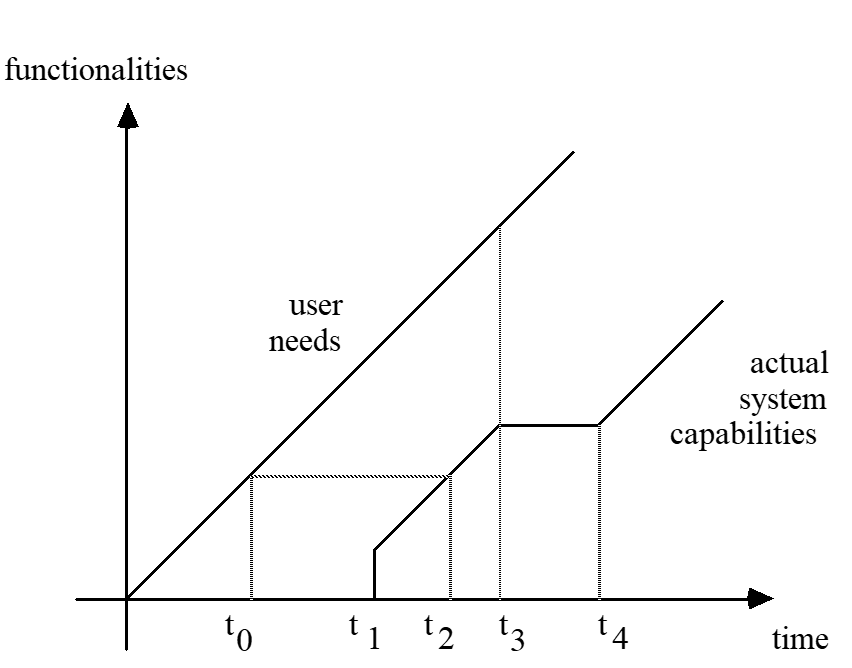
\includegraphics[width=.8\textwidth]{img/timeliness-1.png}
    \end{figure}

    \noindent
    As you can see by the graph, the \dquotes{\emph{user needs}} is a linear function (and sometimes can be exponential!). A software engineer should be able to respond to the client's requests as soon as possible. As the graph shows, a request made on time $t_{0}$ is completed on time $t_{2}$; but another request can be made at that time, and so on. The actual system capabilities can't grow up always because sometimes there are \dquotes{brainstorming times} to increase product quality (ISO/IEC 25010).

    \newpage

    \subsection{Software Lifecycle}

    Initially, no reference model is inside a software lifecycle: code and fix (or refactoring). However, a traditional waterfall model is chosen to react to the many problems that a software engineer faces.
    
    \subsubsection{Waterfall model}
    
    The \definition{waterfall model} is a \textbf{breakdown of development activities into linear sequential phases}, meaning they are passed down onto each other, where each phase depends on the deliverables of the previous one and corresponds to a specialization of tasks.\cite{bomarius2009product} Its organization is the following:
    \begin{itemize}
        \item High phases:
        \begin{itemize}
            \item \underline{\definition{Feasibility Study}}: this is a \textbf{cost-benefit analysis}.
            
            The \textcolor{Red3}{\textbf{\emph{main goal}}} is determining whether the project should be started (e.g. buy or make), possible alternatives, and needed resources. 
            
            The \textcolor{Green4}{\textbf{\emph{outcome}}} is a \textbf{feasibility study document}. This paper provides:
            \begin{itemize}
                \item A preliminary problem description;
                \item Some scenarios describing possible solutions;
                \item Costs and schedules for the different alternatives.
            \end{itemize}


            \item \underline{\definition{Requirements Analysis and Specification}}: this is an \textbf{analysis of the domain in which the application takes place}. 
            
            The \textcolor{Red3}{\textbf{\emph{main goal}}} is to \textbf{identify requirements} and \textbf{derive specifications for the software}. Note these specifics require a (continuous) interaction with the user and an understanding of the properties of the domain. 
            
            The \textcolor{Green4}{\textbf{\emph{outcome}}} is a particular document called \textbf{Requirements Analysis and Specification Document} (RASD).


            \item \underline{\definition{Design}}: this is the \textbf{definition of the software architecture}. There, the definition of components (modules) and the relations/interactions among these components. 
            
            The \textcolor{Red3}{\textbf{\emph{main goal}}} is to \textbf{support the concurrent development of separate responsibilities}. 
            
            The \textcolor{Green4}{\textbf{\emph{outcome}}} is a summary of this info in a \textbf{design document}.
        \end{itemize}

        \item Low phases:
        \begin{itemize}
            \item \underline{\definition{Coding and Unit Test}}: each module is \textbf{implemented using the chosen programming language}. Furthermore, each module is \textbf{tested in isolation} by the module developer. Also, the programs should include their documentation.

            \item \underline{\definition{Integration and System Test}}: the modules are \textbf{integrated into (sub)systems}. The integrated (sub)systems are \textbf{tested}. Follows an incremental implementation scheme. A complete system test is needed to verify the overall properties. Note that sometimes we have alpha test and beta test.

            \item \underline{\definition{Deployment}}: is the process used to conceive, specify, design, program, document, test, and bug fix to create and maintain applications, frameworks, or other software components.

            \item \underline{\definition{Maintenance}}: the maintenance is divided into \textbf{two types}:
            \begin{itemize}
                \item \textbf{Corrective} deals with the \textbf{repair of faults or defects found}.

                \item \textbf{Evolution} is also divided into \textbf{three types}:
                \begin{itemize}
                    \item \textbf{\emph{Adaptive}} maintenance: consists of \textbf{adapting software to changes in the environment} (the hardware or the operating system, business rules, government policies).

                    \item \textbf{\emph{Perfective}} maintenance: mainly deals with accommodating \textbf{new or changed user requirements}.

                    \item \textbf{\emph{Preventive}} maintenance: concerns activities aimed at \textbf{increasing the system's maintainability}.
                \end{itemize}
            \end{itemize}
        \end{itemize}
    \end{itemize}

    \begin{flushleft}
        \textcolor{Red2}{\textbf{\faIcon{exclamation-triangle} Problems derived from correction and evolution}}
    \end{flushleft}
    Note: the \textbf{distinction between correction and evolution can be unclear} because specifications often must be completed and clarified. This causes problems because specs are usually part of a developer and customer contract. 
    \begin{itemize}
        \item \textbf{Early frozen specs} can be problematic because they are more likely to be wrong.
        \item Another problem is \textbf{software evolution} because \textbf{it is never anticipated or planned}. Since the software is easy to change, often, under emergency, changes are applied directly to code, and consequently, the state of project documents is inconsistent.
    \end{itemize}

    \begin{flushleft}
        \textcolor{Green3}{\faIcon{check} \textbf{Solutions - Best practices}}
    \end{flushleft}
    Some good engineering practices exist to solve the evolution problem: \textbf{first, modify the design, then change implementation and apply changes consistently in all documents}. Also, the \textbf{software must be designed to accommodate changes cost-effectively}. This is one of the \emph{main goals} of software engineering.

    \begin{flushleft}
        \textcolor{Green3}{\faIcon{check} \textbf{Flexible processes}}
    \end{flushleft}
    We can make the \textbf{waterfall model more flexible}. In this case, the \textbf{main goal is to adapt to changes (especially in requirements and specs)}.
    The idea is that the stages are \textbf{not necessarily sequential}, and \textbf{processes} become \textbf{iterative and incremental}.

    % TODO: page 9 - 02. Qualities And HPC Software

    \newpage

    \bibliography{bibtex}{}
    \bibliographystyle{plain}

    \newpage

    \printindex
\end{document}